\documentclass[12pt]{report}
\usepackage{auhonors}

\usepackage{ulem}
\usepackage{url}
\usepackage{tikz}
\usepackage{pgf}

% for list of abbreviations
\usepackage[intoc]{nomencl}
\renewcommand{\nomname}{List of Abbreviations}
\makenomenclature
%% don't forget to run:   makeindex ausample.nlo -s nomencl.ist -o ausample.nls

% May want theorems numbered by chapter
\newtheorem{theorem}{Theorem}[chapter]

\title{A Visual Driver Aid and Investigation of Error Propagation in Convoy Following Based on Dynamic Base Real-Time Kinematic Positioning}
\author{Robert Cofield}
\date{May 5, 2013}
\copyrightyear{2013}
\adviser{David Bevly}

\keywords{DRTK, GPS, GUI, Leader-follower, Convoy}

\professor{David Bevly, ...distinctions...}
\professor{Kathie Maddox, ... ...}

\begin{document}

%%%%%%%%%%%%%%%%%%%%%%%%%%%%%%%%%%%%%%%%%%%%%%%%%%%%%%%%%%%%%%%%%%%%%%%%%%%%%%%%
%   Prefatory Pages
%%%%%%%%%%%%%%%%%%%%%%%%%%%%%%%%%%%%%%%%%%%%%%%%%%%%%%%%%%%%%%%%%%%%%%%%%%%%%%%%

\begin{romanpages}

\TitlePage

\begin{abstract}
Abstract
\end{abstract}

\begin{acknowledgments}
Thank people.
\end{acknowledgments}

\tableofcontents
\listoffigures
\listoftables

\printnomenclature[0.75in] 

\end{romanpages}

\normalem       % Make italics the default for \em


%%%%%%%%%%%%%%%%%%%%%%%%%%%%%%%%%%%%%%%%%%%%%%%%%%%%%%%%%%%%%%%%%%%%%%%%%%%%%%%%
%   Chapter 1
%%%%%%%%%%%%%%%%%%%%%%%%%%%%%%%%%%%%%%%%%%%%%%%%%%%%%%%%%%%%%%%%%%%%%%%%%%%%%%%%
\chapter{Introduction}

% Establish the use case
The convoy scenario is examined, wherein a chain of vehicles are aligned front to back along some path determined by the front-most vehicle. Each inner vehicle acts as a leader to that following it, and follows the one preceding it. As such, vehicle must maintain some form of communication with those directly adjacent to it.
The computational tasks for each leader-follower pairing is carried out in the lead vehicle. This is often the ideal setup for other secenarios, such as when the follower is an unmanned aerial vehicle, as UAV's are often limited by weight, and thus outsource processing tasks to ground computers where possible. Relying on the leader for positioning data is even used for swarm setups with a single leader and multiple followers \cite{gian}, regardless of the positioning method. For the present scenario, however, this structure makes the implementation of visualization software for data recieved from each leader much easier to implement with a low computational cost. The following chapter highlights why a navigational aid is necessary for convoy scenarios, why DRTK with TDCP is the ideal solution, and how it functions.

\section{Motivation} %% GET CITATIONS!
%Autonomous scenarios?
% military convoys
The military often uses long trains of transport vehicles to move supplies and munitions through perilous terrain over long distances. Landmines and other explosive roadside devices are common in many combat environments, and a precise path of safe travel may be defined. Rather than use at least one soldier to operate each vehicle, having a single human driver in the lead would reduce manpower and, potentially, casualties in the event that a convoy is attacked. In addition, a machine-driven following vehicle can potentially acheive much greater lateral path following accuracy than a human-driven vehicle.

% commercial trucking
Commercial trucking accounts for XXXXX of all vehicles on the road. In areas where traffic congestion is a serious problem, automation of the driving task could allow for tighter truck groupings, easing congestion and avoiding vehicular collisions. When extremely close together, vehicles experience the aerodynamic phenomenon known as "drafting," whereby the air drag created by a lead vehicle clears the way for those following it, thereby lessening the total force required to propel the vehicle and significantly lowering fuel consumption. In addition, driver "down time"---when truck drivers must rest periodically and stop the vehicle---could almost be eliminated by placing drivers in two to three trucks and having them take turns as the leader of the convoy, resting and allowing the automated following system to control their truck. This would also drastically reduce the labor required to move goods via the highway system

%%%%%%%%%%%%%%%%%%%
% COMPARE SOLUTIONS
\section{Comparison of Positioning Solutions for Real-Time Following}
An abundance of alternatives exist for positioning one vehicle behind another. Many incorporate fusion algorithms, wherein data from multiple sensors providing the same information is intelligently assigned varying weights in the determination of an overall solution. In addition, coupling sensors with complimentary strengths (e.g., IMU and GPS) has proven to be an extremely robust and effective method of localization and navigation \cite{scottthesis}. The following section will overview the strengths and weaknesses of each as a standalone sensor employed for vehicular following as compared DRTK/TDCP.

%%%% RANGING
\subsection{Ranging Devices}
Ranging devices operate on a similar principle to GPS pseudoranging, the time-of-flight. A signal of some type is emitted from the ranging instrument and reflected off some object. Many of the signals return to the ranging device, whereupon the elapsed time is multiplied by the speed of the signal to yield a range. These all require that the object to be detected be visible to the instrument, or have a direct line of sight. While useful in many situations, the present scenario does not always provide for direct line of sight.

% RADAR - finished
The most popular of these technologies is Radio Dectection and Ranging (RADAR), which came to prominence during WWII, and is widely used for adaptive cruise control (ACC) in the automotive industry. The scenario of ACC is similar to the present scenario in that relative positioning is employed to monitor the location of a vehicle travelling directly ahead along a comparable path. The primary goal is to sustain a target forward velocity until doing so would result in a rear-end collision.  RADAR is capable of detecting the kinematic movement of multiple objects within its field of view, but must maintain line-of-sight \cite{lidarvsradaracc}. This does well for avoidance scenarios, but the present objective---while avoiding a rear-end collision is desirable---is quite the opposite.

% SONAR - finished
The simplest implementation of this concept is Sonic Navigation and Ranging (SONAR). Sound waves are emitted and upon return, the calculated distance indicates an object at the determined range somewhere within the field of the emitter. As this provides no orientation, arrays of SONAR devices must often be used to successfully avoid obstacles. This may be combined with odometry to some effect, but navigation is very difficult and highly imprecise.

% LiDAR - finished
Light Detection and Ranging (LiDAR) allows measurement of not only a very precise position, but the optical properties of the detected object. A beam of light is emitted and reflected back to the instrument, whereupon the elapsed time is multiplied by the speed of light to yield a range. For relative positions to be accurate, either mounting of the instrument must be extremely precise or a calibration process is required \cite{jordanlidar}. Once properly tuned, LiDAR may produce errant readings during inclement weather, and also necessitates the adjacent leader to be within line-of-sight for any useable data to be returned. On the other hand, LiDAR also yields a numerical value for the intensity of the objects which are visible, which can be used to determine lateral path deviation provided that lane markings are visible and the path lies within them \cite{cameralidarlane}. 

%%%% VISION
\subsection{Vision}
Convoy following algorithms based on computer vision has existed for quite some time \cite{visionrec}, and like LiDAR lends itself to lane-level positioning, but requires a line-of-sight for any data on the intended leader. Camera systems are also susceptible to direct sunlight, rain, and poor illumination, which in many cases render the system useless. The use of a graphics processing unit is often required, as image processing tasks are computationally expensive, sometimes prohibitively so for embedded systems.
% Mono Camera
A monocular camera employed for the present purposes will typically extract notable features from a rectangular image. To make determination of the leader's pose less error-prone, an easily extractable object of known shape and dimensions can be placed on the rear of the vehicle where it can be seen by the follower camera.
% Stereo Camera
Stereo cameras function much like the human eye, in that depth is obtained from comparing differences between two images of the same object taken simultaneously from two cameras of aligned in parallel at a known separation in the direction perpendicular to the line-of-sight.


%%%%%%%%%%%%%%
% Explain GNSS
\section{Global Navigation Satellite System}

% \subsection{Principles of GNSS}
At the fundamental level, GNSS
\footnote{GNSS is a protocol-agnostic term referring to any of several systems worldwide which use satellites to provide a receiver on the ground with position information. The US implementation is known as GPS, the Russian positioning system is referred to as GLONASS, and the European Union has Galileo.}
comprises a constellation of orbitting satellites whose positions above the earth are known, corresponding with a receiver to give as many range measurements as possible so that a global 3 dimensional location may be calculated. GNSS does not necessitate line of sight, and is not impaired by lighting effects, though a clear view of the sky is needed to connect to as many satellites as possible. The range for highly accurate following is large, on the order of kilometers depending upon speed, and lower accuracy following can be performed for two vehicles at any distance. These make GNSS ideal for use in the leader-follower convoy scenario.

% \subsection{Relevant Improvements to Standalone GPS}
% RTK - finished
Oftentimes, when working in a defined area, the exact location of a nearby point is known. If this is not the case, the exact location of a point may be found by setting up a static GPS receiver and allowing the measurements to average towards zero error over a long period of time. Once the precise location is known, the base station can transmit the difference between this value and the position received by standalone GPS to nearby receivers in real-time. Using these corrections to compensate for errors is known as Real Time Kinematic (RTK) GPS. It produces extremely accurate global positioning (i.e., in the earth coordinate frame).
% DRTK
RTK assumes that two receivers will experience similar errors when in close proximity and measuring simultaneously. The same principal applies to two receivers when both are kinematically active, but a globally accurate position is no longer possible without some reference. Instead, a high-accuracy relative position vector (RPV) can be obtained by subtracting the position of one receiver from that another at the same time epoch.
% TDCP
This practice of subtracting errors can be extended to work with a single receiver. Between very successive measurment epochs taken in short periods, many of the errors in standard GPS remain constant. The corresponding time difference of the carrier phase (TDCP) can then be used to calculate a change in position between time steps, also known as odometry \cite{travisdiss}.


%%%%%%%%%%%%%%%%%%%%%%%%%%%%%%%%%
% How we get what's on the screen
\section{Position Using the DRTK and TDCP Algorithms}
Figure \ref{fig:drtktdcp} illustrates how information is taken from each receiver to obtain the information necessary for the display. The algorithms used to calculate information displayed by the GUI have been developed extensively by \cite{scottthesis},\cite{travisshort}, \cite{travisconvoy} and \cite{travisdiss}. The Driver Assisted Following (DAF) algorithm adds odometry from the TDCP algorithm to RPVs from the DRTK algorithm to obtain a set of points in the East-North-Up (ENU) coordinate frame---with the origin at the follower---which lie along the path taken by the leader. Distance between relative path points depends upon the velocity of the leader and the frequency of the slowest algorithm. The specifications of all hardware used are outlined in Chapter \ref{chap:exper}.

% flowchart - How the data gets from receiver to gui
\begin{figure}[htbp]
    \centering
    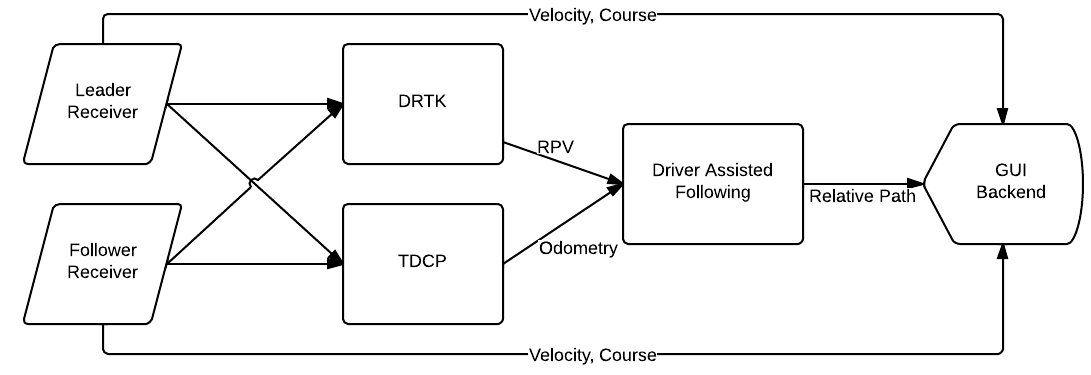
\includegraphics[width=6.5in]{./figs/data_algo.png}
    \caption{Relative path determination processes}
    \label{fig:drtktdcp}
\end{figure}

%%%% ACCURACY
% \subsection{Accuracy}
% \label{sec:theoacc}
% DRTK accuracy - finished
The accuracy of DRTK GPS is primarily contingent upon the availability of dual-band (L1 and L2, rather than L1 only) signals, and of high precision ambiguity estimates (fixed integer rather than floating point). Under ideal conditions, the root-mean-square error of DRTK positions will be as low as $0.33~cm$ with a variance of $0.10~cm^2$. 
% TDCP accuracy 
The accuracy of the TDCP algorithm decreases over time as errors in the position changes accumulate. The mean time for a static receiver to accumulate $1.0~m$ lateral error is $378~s$, so the curvilinear distance at which this error will be present is contingent upon the speed of the follower. A complete analysis of the DRTK/TDCP algorithm error behavior is provided by \cite{scottthesis}. The combined accuracy traits of the system when employed for convoys of three or more vehicles are explored in Chapter \ref{chap:errprop}.



%%%%%%%%%%%%%%%%%%%%%%%%%%%%%%%%%%%%%%%%%%%%%%%%%%%%%%%%%%%%%%%%%%%%%%%%%%%%%%%%
%   Chapter 2
%%%%%%%%%%%%%%%%%%%%%%%%%%%%%%%%%%%%%%%%%%%%%%%%%%%%%%%%%%%%%%%%%%%%%%%%%%%%%%%%
\chapter{Graphical User Interface}

%%%%%%%%%%%%%%%%%%%%%%
% Architecture Section
\section{Architecture}
Figure \ref{fig:blackboxflow} depicts the predefined inputs and outputs of the GUI.

% Black box info flow chart
\begin{figure}[htbp]
    \centering
    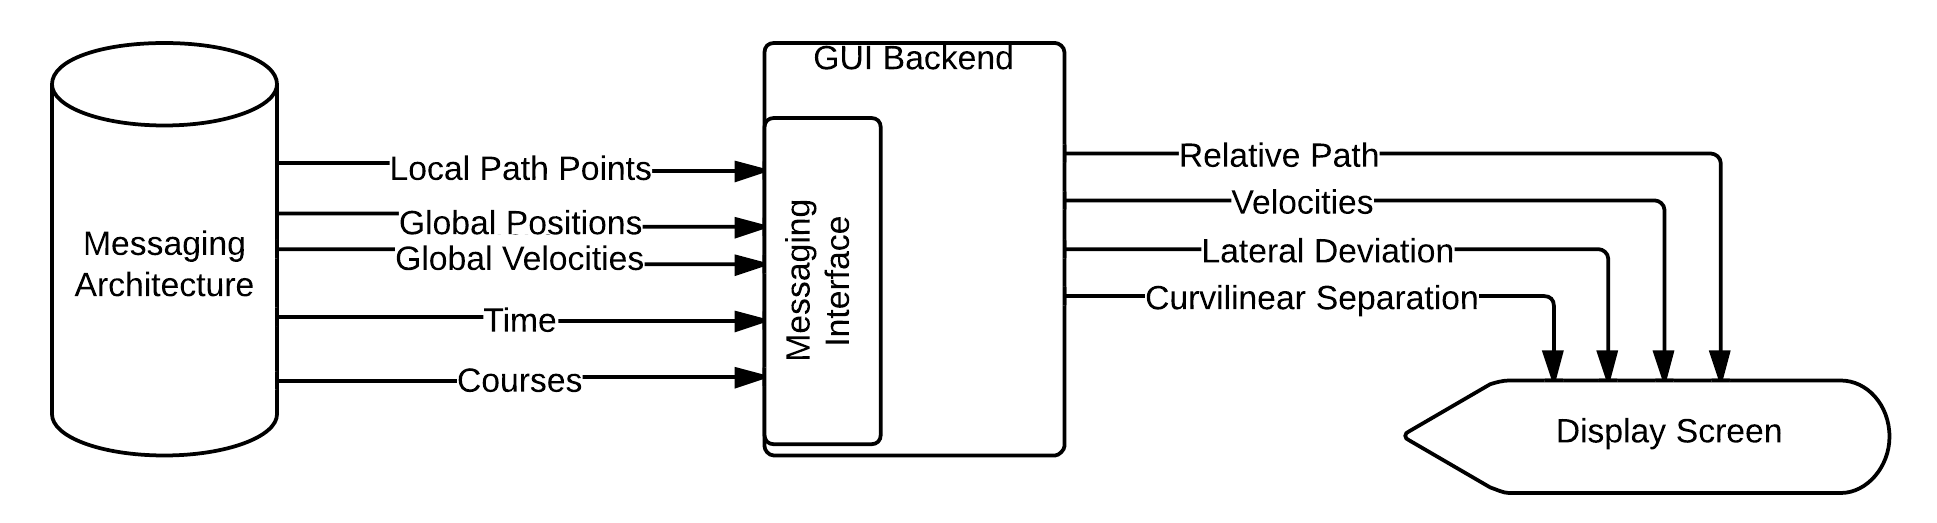
\includegraphics[width=6.5in]{./figs/blackbox_flowchart.png}
    \caption{Information flow architecture}
    \label{fig:blackboxflow}
\end{figure}

\subsection{Message Passing}
The primary message passing architecture used was the Mission Oriented Operating Suite (MOOS), as developed by \cite{moos}.

%%%%%%%%%%%%%%%%%%%%%%
% Final Design Section
\section{Final Design}
The end user---the driver---will primarily be presented with the screen depicted in Fig. \ref{fig:finaldesdriv}. There is always the option to change operational parameters, using the screen depicted in Figure \ref{fig:finaldesopts}.

% the driver screen
\begin{figure}[htbp]
    \centering
    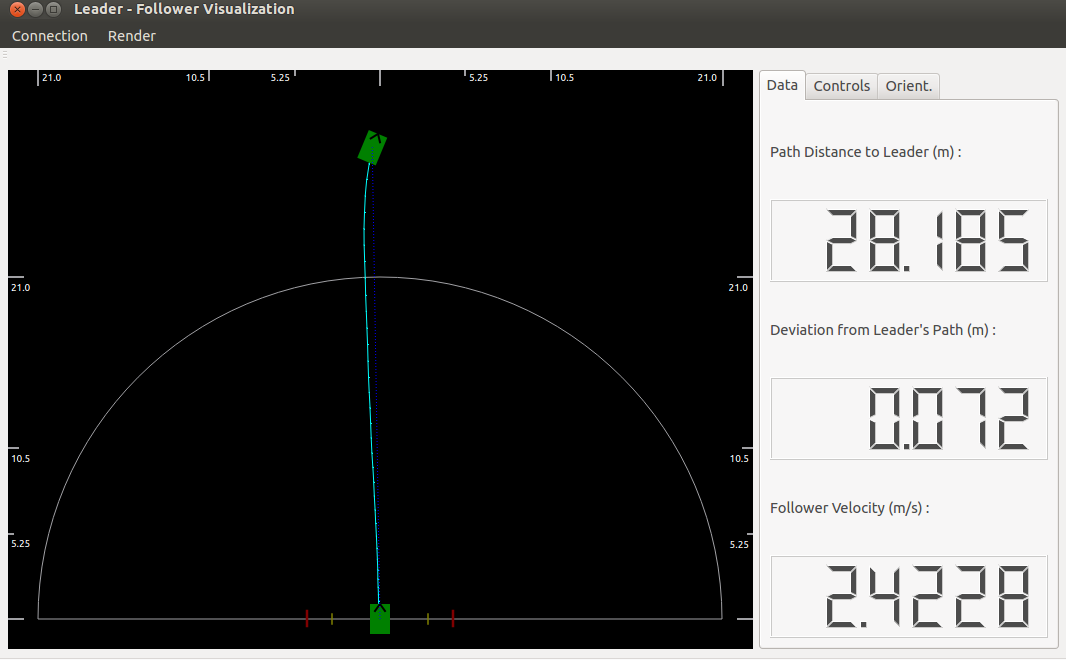
\includegraphics[width=6.5in]{./figs/final_design_data.png}
    \caption{Final Design --- Driver view}
    \label{fig:finaldesdriv}
\end{figure}

% the option screen
\begin{figure}[htbp]
    \centering
    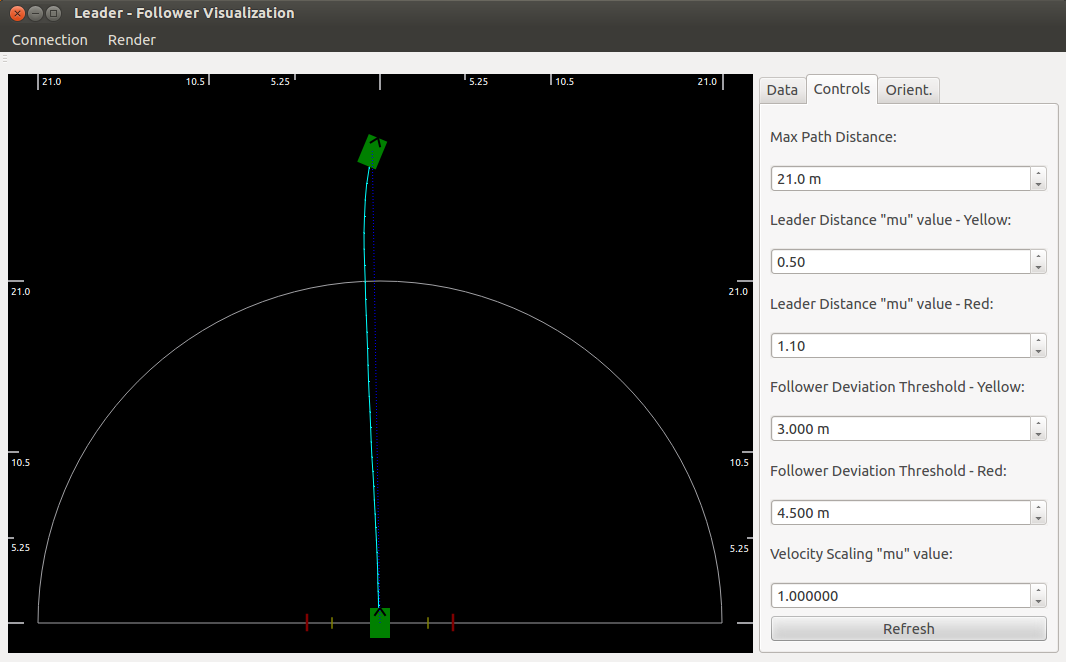
\includegraphics[width=6.5in]{./figs/final_design_opts.png}
    \caption{Final Design --- Setting of operational parameters }
    \label{fig:finaldesopts}
\end{figure}


%%%%%%%%%%%%%%%%%%%%%%%%%%%%%%%%%%%%%%%%%%%%%%%%%%%%%%%%%%%%%%%%%%%%%%%%%%%%%%%%
%   Chapter 3
%%%%%%%%%%%%%%%%%%%%%%%%%%%%%%%%%%%%%%%%%%%%%%%%%%%%%%%%%%%%%%%%%%%%%%%%%%%%%%%%
\chapter{Experimentation}
\label{chap:exper}


%%%%%%%%%%%%%%%%%%%%%%%%%%%%%%%%%%%%%%%%%%%%%%%%%%%%%%%%%%%%%%%%%%%%%%%%%%%%%%%%
%   Chapter 4
%%%%%%%%%%%%%%%%%%%%%%%%%%%%%%%%%%%%%%%%%%%%%%%%%%%%%%%%%%%%%%%%%%%%%%%%%%%%%%%%
\chapter{Error Propagation in Convoys}
\label{chap:errprop}


%%%%%%%%%%%%%%%%%%%%%%%%%%%%%%%%%%%%%%%%%%%%%%%%%%%%%%%%%%%%%%%%%%%%%%%%%%%%%%%%
%   Chapter 5
%%%%%%%%%%%%%%%%%%%%%%%%%%%%%%%%%%%%%%%%%%%%%%%%%%%%%%%%%%%%%%%%%%%%%%%%%%%%%%%%
\chapter{Conclusions}


%%%%%%%%%%%%%%%%%%%%%%%%%%%%%%%%%%%%%%%%%%%%%%%%%%%%%%%%%%%%%%%%%%%%%%%%%%%%%%%%
%   Bib
%%%%%%%%%%%%%%%%%%%%%%%%%%%%%%%%%%%%%%%%%%%%%%%%%%%%%%%%%%%%%%%%%%%%%%%%%%%%%%%%
\bibliographystyle{asmems4}
\bibliography{thesis}

\nocite{travisdiss}
\nocite{travisshort}
% \bibitem{travismartin} William Travis, Scott Martin and David M. Bevly, ``Automated short distance vehicle following using a dynamic base RTK system." Int. J. Vehicle Autonomous Systems, Vol. 9, Nos. 1/2, 2011. pp 126-141

% \bibitem{platoon} M. E. Cannon, C. Basnayake, S. Syed, and G. Lachapelle. ``Precise gps sensor subsystem for Vehicle Platoon  Control." In Proceedings of ION GPS/GNSS 2003 Conference. pp 213-224, 2003.

\end{document}